
\documentclass[12pt]{article}
\usepackage{jwstproposaltemplate}
\usepackage{hyperref}
\usepackage{graphicx}
\usepackage[subpreambles=true]{standalone}
\usepackage{caption}
\usepackage{subcaption}

\begin{document}

\begin{figure}
     \centering
     \begin{subfigure}[b]{0.4\textwidth}
         \centering
         \includegraphics[width=\textwidth]{figs/H.pdf}
         \caption{$y=x$}
         \label{fig:y equals x}
     \end{subfigure}
     \hfill
     \begin{subfigure}[b]{0.4\textwidth}
         \centering
         \includegraphics[width=\textwidth]{figs/ch1.pdf}
         \caption{$y=3sinx$}
         \label{fig:three sin x}
     \end{subfigure}
        \caption{Three simple graphs}
        \label{fig:three graphs}
\end{figure}


\begin{figure}
     \centering
     \begin{subfigure}[b]{0.3\textwidth}
         \centering
         \includegraphics[width=1.2\textwidth]{figs/dz_WAFLS_const.pdf}
         \caption{$y=x$}
         \label{fig:y equals x}
     \end{subfigure}
     \hfill
     \begin{subfigure}[b]{0.3\textwidth}
         \centering
         \includegraphics[width=1.2\textwidth]{figs/dz_WAFLS_inst.pdf}
         \caption{$y=3sinx$}
         \label{fig:three sin x}
     \end{subfigure}
     \begin{subfigure}[b]{0.3\textwidth}
         \caption{This is a side caption.}
     \end{subfigure}
        \caption{Three simple graphs}
        \label{fig:three graphs}
\end{figure}


\begin{figure}
     \centering
     \begin{subfigure}[b]{0.7\textwidth}
         \centering
         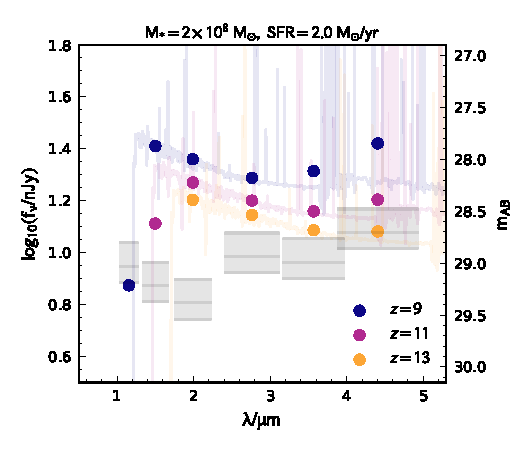
\includegraphics[width=\textwidth]{figs/SED.pdf}
         \caption{$y=x$}
         \label{fig:y equals x}
     \end{subfigure}
\end{figure}


\begin{figure}
     \centering
     \begin{subfigure}[b]{0.7\textwidth}
         \centering
         \includegraphics[width=\textwidth]{figs/WAFLS.pdf}
         \caption{$y=x$}
         \label{fig:y equals x}
     \end{subfigure}
\end{figure}


\begin{figure}
     \centering
     \begin{subfigure}[b]{0.4\textwidth}
         \centering
         \includegraphics[width=\textwidth]{figs/LF_simple_multi_10.pdf}
         \caption{$y=x$}
         \label{fig:y equals x}
     \end{subfigure}
     \hfill
     \begin{subfigure}[b]{0.4\textwidth}
         \centering
         \includegraphics[width=\textwidth]{figs/LF_simple_multi_11.pdf}
         \caption{$y=3sinx$}
         \label{fig:three sin x}
     \end{subfigure}
        \caption{Three simple graphs}
        \label{fig:three graphs}
\end{figure}

\begin{figure}
     \centering
     \begin{subfigure}[b]{0.7\textwidth}
         \centering
         \includegraphics[width=\textwidth]{figs/surface_densities.png}
         \caption{$y=x$}
         \label{fig:y equals x}
     \end{subfigure}
\end{figure}


\end{document}